\section{\emph{Code-Survey} Methodology}
\label{sec:methodology}

This section outlines the \emph{Code-Survey} methodology, which integrates the expertise of human participants and the efficiency of Large Language Model (LLM) agents to convert unstructured software data—such as commit histories and mailing lists—into structured datasets suitable for analysis.

The central principle behind \emph{Code-Survey} is to treat LLMs as human participants in a survey-like process. While LLMs can process data more quickly and at lower costs than humans, they are also prone to errors, guesses, and limitations in specific domains, much like human participants~\cite{ji2023survey}. By leveraging traditional survey methodologies designed for humans, we can efficiently conduct LLM-based surveys while maintaining oversight and validation from human experts. Additionally, LLM agents can utilize traditional tools to automate analysis tasks.

\begin{figure}[t]
    \centering
    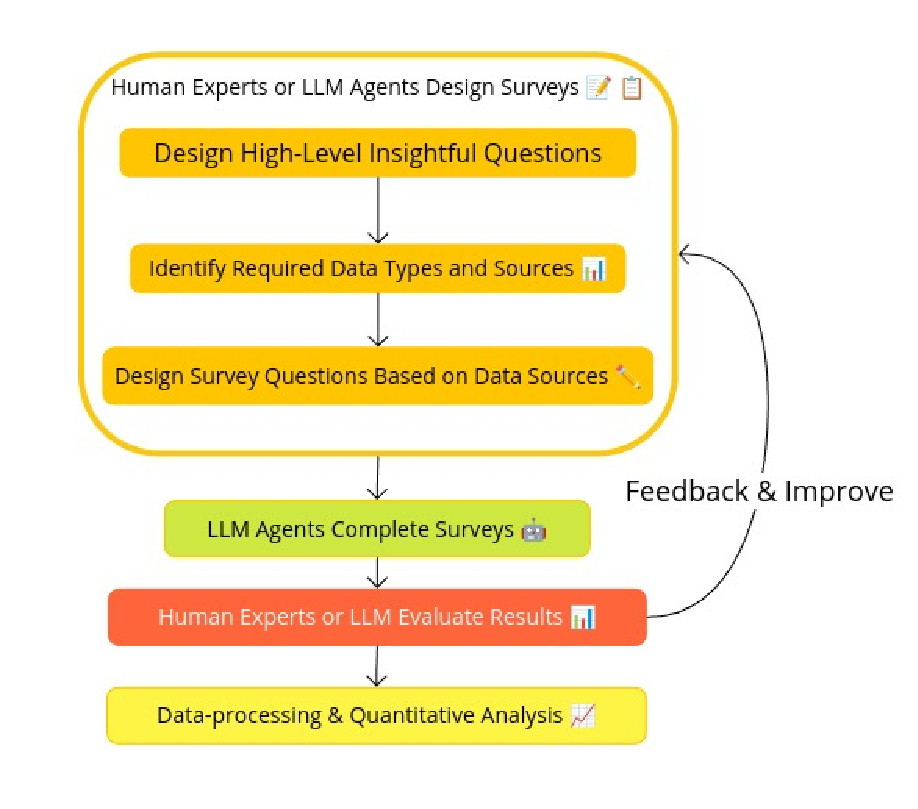
\includegraphics[width=0.5\textwidth]{workflow.pdf}
    \caption{\emph{Code-Survey} Workflow}
    \label{fig:workflow}
\end{figure}

\subsection{Workflow}

The \emph{Code-Survey} process follows a structured workflow, as illustrated in Figure~\ref{fig:workflow}:

\begin{enumerate}
    \item \textbf{Survey Design by Human Experts or LLM Agents}: Experts or LLM agents create tailored questions for each type of unstructured data (e.g., commits, emails) to extract key insights. The survey design is crucial for guiding the LLM in structuring the data effectively and focuses on tasks aligned with the LLM's strengths, such as summarization and yes/no questions. This step should minimizes the usage of open-ended questions that require deep domain expertise.

    \item \textbf{Survey Completion by LLM Agents}: LLM agents process the unstructured input by answering the survey questions. They organize data into structured formats by tagging relevant information, summarizing key points, and identifying important patterns. This step is fundamental in transforming unstructured data into structured datasets, enabling more straightforward analysis.

    \item \textbf{Evaluation of Survey Results by Human Experts or LLM Agents}: Human experts with domain-specific knowledge, or additional LLM agents, evaluate a sample of the structured data. This evaluation ensures accuracy and allows for the detection of discrepancies. If the results are unsatisfactory, the process loops back to Step 1, where the survey design is refined.

    \item \textbf{Data Processing and Quantitative Analysis}: The structured data undergoes further processing to analyze key metrics and patterns. Quantitative analysis is performed to identify trends in development, feature interdependencies, and areas needing improvement in reliability and security. This provides a detailed view of the system's evolution and characteristics.

\end{enumerate}

This process employs an iterative design, allowing surveys to be refined based on analysis results, thereby creating a feedback loop that enhances data structuring and interpretation. By leveraging both LLMs and human oversight, the \emph{Code-Survey} methodology efficiently handles large volumes of unstructured software data. At each step, human experts can interactively contribute, or LLM agents can automate the process.

\subsection{Survey Design with LLM Assistance}

A key aspect of \emph{Code-Survey} is designing effective surveys to generate accurate data. Surveys can be designed by humans or LLM agents. We identify three key steps to guide LLM agents in designing surveys. The following prompts serve as a framework or LLM input for survey creation:

\begin{enumerate}
    \item \textbf{Design High-Level Insightful Questions}: If you could ask every kernel developer to complete a survey or questionnaire about a commit or an email, what are the most insightful questions related to design, implementation, maintenance, reliability, and security? Describe the possible questions in detail.

    \item \textbf{Identify Required Data Types and Sources}: What data types and sources are required to answer the insightful questions described previously? Describe the data types and sources for each question in detail.

    \item \textbf{Design Survey Questions to Retrieve Data}: What survey questions can you design to obtain the required data types for the insightful questions from the data sources described previously? Describe the survey questions for kernel developers in detail.

\end{enumerate}

This workflow ensures that the LLM-driven survey design process leads to structured data that offers deeper insights into complex software systems, such as the Linux kernel. By guiding LLM agents through these steps, we can systematically extract valuable information from unstructured data sources.
